%! TeX program = lualatex
\documentclass[a4paper,12pt,article]{memoir}
% TeX root=../main.tex

\settrimmedsize{\stockheight}{\stockwidth}{*}
\settypeblocksize{220mm}{130mm}{*}
\setlrmargins{*}{*}{1.7}
\setulmargins{30mm}{*}{*}
\setmarginnotes{20pt}{100pt}{10pt}
\checkandfixthelayout%

% \setsidefeet{\marginparsep}{\marginparwidth}%
% {0.8\onelineskip}{0pt}%
% {\normalfont\footnotesize}{\textheight}%
\setsidecaps{\marginparsep}{\marginparwidth}
\setlength{\footmarkwidth}{0.5em}
\setlength{\footmarksep}{0em}
\setlength{\footparindent}{0em}
\footmarkstyle{\textsuperscript{#1}\hspace{0.5em}}

\makeoddfoot{plain}{}{}{\thepage}
\makeevenfoot{plain}{\thepage}{}{}
\makepagestyle{ruled}
\makeevenfoot{ruled}{\thepage}{}{} % page numbers at the outside
\makeoddfoot{ruled}{}{}{\thepage}
\makeheadrule{ruled}{\textwidth}{0.75pt}
\makeevenhead{ruled}{\scshape\leftmark}{}{}
\makeoddhead{ruled}{}{}{\scshape\rightmark}
\makepsmarks{ruled}{%
	\nouppercaseheads%
	\createmark{chapter}{left}{shownumber}{\scshape}{.\space}
	\createmark{part}{right}{shownumber}{}{.\space}
	\createmark{section}{right}{shownumber}{}{.\space}
	\createmark{subsection}{right}{shownumber}{}{.\space}
	\createplainmark{toc}{both}{\contentsname}
	\createplainmark{lof}{both}{\listfigurename}
	\createplainmark{lot}{both}{\listtablename}
	\createplainmark{bib}{both}{\bibname}
	\createplainmark{index}{both}{\indexname}
	\createplainmark{glossary}{both}{\glossaryname}
}

% decorando divisões
\setsecnumdepth{subsection}
\setcounter{tocdepth}{3}
\newcommand\chap[1]{%
	\chapter*[#1]{#1}%
	\addcontentsline{toc}{chapter}{#1}}


% paleta de cores
\usepackage{xcolor}
\definecolor{green}{rgb}{16,87,87} % rgb(16,87,87)
\definecolor{red}{rgb}{193, 11, 105} % rgb(193, 11, 105)
\definecolor{yellow}{rgb}{218,222,104} % rgb(218,222,104)
\definecolor{pink}{rgb}{243,179,145} % rgb(243,179,145)
\definecolor{blue}{rgb}{161,184,206} % rgb(161,184,206)

\usepackage[tracking=true]{microtype}

\usepackage{scalefnt}


\usepackage{paralist}
\usepackage{graphicx}
\usepackage{subcaption}
\usepackage{linguex}
\usepackage{multicol}

\usepackage{hyperref}%
\hypersetup{%
	colorlinks=true, % false: boxed links; true: colored links
	linkcolor=green,  % color of internal links
	citecolor=green,  % color of links to bibliography
	filecolor=pink,  % color of file links
	urlcolor=green,
}
% Configurações para o autoref
\renewcommand{\figureautorefname}{Figura}
\renewcommand{\tableautorefname}{Tabela}
\renewcommand{\sectionautorefname}{Seção}
\renewcommand{\chapterautorefname}{Capítulo}
\renewcommand{\subsectionautorefname}{Subseção}


\directlua{dofile('./utils/pie.lua')}
\newcommand{\hittitetrans}[1]{%
  \directlua{hittite_transcription("#1")}}
\newcommand{\luwiantrans}[1]{%
  \directlua{luwian_transcription("#1")}}
\newcommand{\pietrans}[1]{%
  \directlua{pie_transcription("#1")}}

\newcommand{\Prep}{{\footnotesize\textsc{Prep.}}}
\newcommand{\Det}{{\footnotesize\textsc{Det.}}}
\newcommand{\Clt}{{\footnotesize\textsc{Clt.}}}
\newcommand{\Nom}{{\footnotesize\textsc{Nom.}}}
\newcommand{\Acu}{{\footnotesize\textsc{Acu.}}}
\newcommand{\Dat}{{\footnotesize\textsc{Dat.}}}
\newcommand{\Gen}{{\footnotesize\textsc{Gen.}}}
\newcommand{\Abl}{{\footnotesize\textsc{Abl.}}}
\newcommand{\Sg}{{\footnotesize\textsc{Sg.}}}
\newcommand{\Pl}{{\footnotesize\textsc{Pl.}}}
\newcommand{\Com}{{\footnotesize\textsc{Com.}}}
\newcommand{\Neut}{{\footnotesize\textsc{Neut.}}}
\newcommand{\Rel}{{\footnotesize\textsc{Rel.}}}
\newcommand{\Conj}{{\footnotesize\textsc{Conj.}}}
\newcommand{\Pret}{{\footnotesize\textsc{Pret.}}}
\newcommand{\Pro}{{\footnotesize\textsc{Pro.}}}
\newcommand{\Refl}{{\footnotesize\textsc{Refl.}}}
\newcommand{\La}[1]{\textsc{l}.#1}

\usepackage{csquotes}
\usepackage{fontspec}
\usepackage[main=brazil]{babel}
\defaultfontfeatures{Renderer=Harfbuzz}

\babelfont[brazil]{rm}[
	SmallCapsFont=Gentium Plus,
	SmallCapsFeatures={Letters=SmallCaps}]{Crimson Pro}
\babelfont[brazil]{sf}{Noto Sans}
\babelfont[brazil]{tt}[Scale=0.8]{Mononoki Nerd Font}

\babelfont[german]{rm}[
	SmallCapsFont=Gentium Plus,
	SmallCapsFeatures={Letters=SmallCaps}]{Crimson Pro}
\babelfont[brazil]{sf}{Noto Sans}
\babelfont[brazil]{tt}[Scale=0.8]{Mononoki Nerd Font}

\babelfont[english]{rm}[
	SmallCapsFont=Gentium Plus,
	SmallCapsFeatures={Letters=SmallCaps}]{Crimson Pro}
\babelfont[english]{sf}{Noto Sans}
\babelfont[english]{tt}[Scale=0.8]{Mononoki Nerd Font}

\babelfont[german]{rm}[
	SmallCapsFont=Gentium Plus,
	SmallCapsFeatures={Letters=SmallCaps}]{Crimson Pro}
\babelfont[german]{sf}{Noto Sans}
\babelfont[german]{tt}[Scale=0.8]{Mononoki Nerd Font}


\babelprovide[import, onchar=ids fonts letters]{ancientgreek}
\babelfont[ancientgreek]{rm}{Brill}
\babeltags{grc = ancientgreek}

\babelprovide[import]{hebrew}
\babelfont[hebrew]{rm}[Scale=0.8]{Ezra SIL}

\babelprovide[onchar=ids fonts]{luwian}
\babelfont[luwian]{rm}[
	SmallCapsFont=Gentium Plus,
Script=Anatolian Hieroglyphs]{Noto Sans Anatolian Hieroglyphs}
\babelfont[luwian]{sf}[
	SmallCapsFont=Gentium Plus,
Script=Anatolian Hieroglyphs]{Noto Sans Anatolian Hieroglyphs}
\babelcharproperty{`𔐀}{locale}{luwian}
\babelcharproperty{`𔐁}{locale}{luwian}
\babelcharproperty{`𔐂}{locale}{luwian}
\babelcharproperty{`𔐃}{locale}{luwian}
\babelcharproperty{`𔐄}{locale}{luwian}
\babelcharproperty{`𔐅}{locale}{luwian}
\babelcharproperty{`𔐆}{locale}{luwian}
\babelcharproperty{`𔐇}{locale}{luwian}
\babelcharproperty{`𔐈}{locale}{luwian}
\babelcharproperty{`𔐉}{locale}{luwian}
\babelcharproperty{`𔐊}{locale}{luwian}
\babelcharproperty{`𔐋}{locale}{luwian}
\babelcharproperty{`𔐌}{locale}{luwian}
\babelcharproperty{`𔐍}{locale}{luwian}
\babelcharproperty{`𔐎}{locale}{luwian}
\babelcharproperty{`𔐏}{locale}{luwian}
\babelcharproperty{`𔐐}{locale}{luwian}
\babelcharproperty{`𔐑}{locale}{luwian}
\babelcharproperty{`𔐒}{locale}{luwian}
\babelcharproperty{`𔐓}{locale}{luwian}
\babelcharproperty{`𔐔}{locale}{luwian}
\babelcharproperty{`𔐕}{locale}{luwian}
\babelcharproperty{`𔐖}{locale}{luwian}
\babelcharproperty{`𔐗}{locale}{luwian}
\babelcharproperty{`𔐘}{locale}{luwian}
\babelcharproperty{`𔐙}{locale}{luwian}
\babelcharproperty{`𔐚}{locale}{luwian}
\babelcharproperty{`𔐛}{locale}{luwian}
\babelcharproperty{`𔐜}{locale}{luwian}
\babelcharproperty{`𔐝}{locale}{luwian}
\babelcharproperty{`𔐞}{locale}{luwian}
\babelcharproperty{`𔐟}{locale}{luwian}
\babelcharproperty{`𔐠}{locale}{luwian}
\babelcharproperty{`𔐡}{locale}{luwian}
\babelcharproperty{`𔐢}{locale}{luwian}
\babelcharproperty{`𔐣}{locale}{luwian}
\babelcharproperty{`𔐤}{locale}{luwian}
\babelcharproperty{`𔐥}{locale}{luwian}
\babelcharproperty{`𔐦}{locale}{luwian}
\babelcharproperty{`𔐧}{locale}{luwian}
\babelcharproperty{`𔐨}{locale}{luwian}
\babelcharproperty{`𔐩}{locale}{luwian}
\babelcharproperty{`𔐪}{locale}{luwian}
\babelcharproperty{`𔐫}{locale}{luwian}
\babelcharproperty{`𔐬}{locale}{luwian}
\babelcharproperty{`𔐭}{locale}{luwian}
\babelcharproperty{`𔐮}{locale}{luwian}
\babelcharproperty{`𔐯}{locale}{luwian}
\babelcharproperty{`𔐰}{locale}{luwian}
\babelcharproperty{`𔐱}{locale}{luwian}
\babelcharproperty{`𔐲}{locale}{luwian}
\babelcharproperty{`𔐳}{locale}{luwian}
\babelcharproperty{`𔐴}{locale}{luwian}
\babelcharproperty{`𔐵}{locale}{luwian}
\babelcharproperty{`𔐶}{locale}{luwian}
\babelcharproperty{`𔐷}{locale}{luwian}
\babelcharproperty{`𔐸}{locale}{luwian}
\babelcharproperty{`𔐹}{locale}{luwian}
\babelcharproperty{`𔐺}{locale}{luwian}
\babelcharproperty{`𔐻}{locale}{luwian}
\babelcharproperty{`𔐼}{locale}{luwian}
\babelcharproperty{`𔐽}{locale}{luwian}
\babelcharproperty{`𔐾}{locale}{luwian}
\babelcharproperty{`𔐿}{locale}{luwian}
\babelcharproperty{`𔑀}{locale}{luwian}
\babelcharproperty{`𔑁}{locale}{luwian}
\babelcharproperty{`𔑂}{locale}{luwian}
\babelcharproperty{`𔑃}{locale}{luwian}
\babelcharproperty{`𔑄}{locale}{luwian}
\babelcharproperty{`𔑅}{locale}{luwian}
\babelcharproperty{`𔑆}{locale}{luwian}
\babelcharproperty{`𔑇}{locale}{luwian}
\babelcharproperty{`𔑈}{locale}{luwian}
\babelcharproperty{`𔑉}{locale}{luwian}
\babelcharproperty{`𔑊}{locale}{luwian}
\babelcharproperty{`𔑋}{locale}{luwian}
\babelcharproperty{`𔑌}{locale}{luwian}
\babelcharproperty{`𔑍}{locale}{luwian}
\babelcharproperty{`𔑎}{locale}{luwian}
\babelcharproperty{`𔑏}{locale}{luwian}
\babelcharproperty{`𔑐}{locale}{luwian}
\babelcharproperty{`𔑑}{locale}{luwian}
\babelcharproperty{`𔑒}{locale}{luwian}
\babelcharproperty{`𔑓}{locale}{luwian}
\babelcharproperty{`𔑔}{locale}{luwian}
\babelcharproperty{`𔑕}{locale}{luwian}
\babelcharproperty{`𔑖}{locale}{luwian}
\babelcharproperty{`𔑗}{locale}{luwian}
\babelcharproperty{`𔑘}{locale}{luwian}
\babelcharproperty{`𔑙}{locale}{luwian}
\babelcharproperty{`𔑚}{locale}{luwian}
\babelcharproperty{`𔑛}{locale}{luwian}
\babelcharproperty{`𔑜}{locale}{luwian}
\babelcharproperty{`𔑝}{locale}{luwian}
\babelcharproperty{`𔑞}{locale}{luwian}
\babelcharproperty{`𔑟}{locale}{luwian}
\babelcharproperty{`𔑠}{locale}{luwian}
\babelcharproperty{`𔑡}{locale}{luwian}
\babelcharproperty{`𔑢}{locale}{luwian}
\babelcharproperty{`𔑣}{locale}{luwian}
\babelcharproperty{`𔑤}{locale}{luwian}
\babelcharproperty{`𔑥}{locale}{luwian}
\babelcharproperty{`𔑦}{locale}{luwian}
\babelcharproperty{`𔑧}{locale}{luwian}
\babelcharproperty{`𔑨}{locale}{luwian}
\babelcharproperty{`𔑩}{locale}{luwian}
\babelcharproperty{`𔑪}{locale}{luwian}
\babelcharproperty{`𔑫}{locale}{luwian}
\babelcharproperty{`𔑬}{locale}{luwian}
\babelcharproperty{`𔑭}{locale}{luwian}
\babelcharproperty{`𔑮}{locale}{luwian}
\babelcharproperty{`𔑯}{locale}{luwian}
\babelcharproperty{`𔑰}{locale}{luwian}
\babelcharproperty{`𔑱}{locale}{luwian}
\babelcharproperty{`𔑲}{locale}{luwian}
\babelcharproperty{`𔑳}{locale}{luwian}
\babelcharproperty{`𔑴}{locale}{luwian}
\babelcharproperty{`𔑵}{locale}{luwian}
\babelcharproperty{`𔑶}{locale}{luwian}
\babelcharproperty{`𔑷}{locale}{luwian}
\babelcharproperty{`𔑸}{locale}{luwian}
\babelcharproperty{`𔑹}{locale}{luwian}
\babelcharproperty{`𔑺}{locale}{luwian}
\babelcharproperty{`𔑻}{locale}{luwian}
\babelcharproperty{`𔑼}{locale}{luwian}
\babelcharproperty{`𔑽}{locale}{luwian}
\babelcharproperty{`𔑾}{locale}{luwian}
\babelcharproperty{`𔑿}{locale}{luwian}
\babelcharproperty{`𔒀}{locale}{luwian}
\babelcharproperty{`𔒁}{locale}{luwian}
\babelcharproperty{`𔒂}{locale}{luwian}
\babelcharproperty{`𔒃}{locale}{luwian}
\babelcharproperty{`𔒄}{locale}{luwian}
\babelcharproperty{`𔒅}{locale}{luwian}
\babelcharproperty{`𔒆}{locale}{luwian}
\babelcharproperty{`𔒇}{locale}{luwian}
\babelcharproperty{`𔒈}{locale}{luwian}
\babelcharproperty{`𔒉}{locale}{luwian}
\babelcharproperty{`𔒊}{locale}{luwian}
\babelcharproperty{`𔒋}{locale}{luwian}
\babelcharproperty{`𔒌}{locale}{luwian}
\babelcharproperty{`𔒍}{locale}{luwian}
\babelcharproperty{`𔒎}{locale}{luwian}
\babelcharproperty{`𔒏}{locale}{luwian}
\babelcharproperty{`𔒐}{locale}{luwian}
\babelcharproperty{`𔒑}{locale}{luwian}
\babelcharproperty{`𔒒}{locale}{luwian}
\babelcharproperty{`𔒓}{locale}{luwian}
\babelcharproperty{`𔒔}{locale}{luwian}
\babelcharproperty{`𔒕}{locale}{luwian}
\babelcharproperty{`𔒖}{locale}{luwian}
\babelcharproperty{`𔒗}{locale}{luwian}
\babelcharproperty{`𔒘}{locale}{luwian}
\babelcharproperty{`𔒙}{locale}{luwian}
\babelcharproperty{`𔒚}{locale}{luwian}
\babelcharproperty{`𔒛}{locale}{luwian}
\babelcharproperty{`𔒜}{locale}{luwian}
\babelcharproperty{`𔒝}{locale}{luwian}
\babelcharproperty{`𔒞}{locale}{luwian}
\babelcharproperty{`𔒟}{locale}{luwian}
\babelcharproperty{`𔒠}{locale}{luwian}
\babelcharproperty{`𔒡}{locale}{luwian}
\babelcharproperty{`𔒢}{locale}{luwian}
\babelcharproperty{`𔒣}{locale}{luwian}
\babelcharproperty{`𔒤}{locale}{luwian}
\babelcharproperty{`𔒥}{locale}{luwian}
\babelcharproperty{`𔒦}{locale}{luwian}
\babelcharproperty{`𔒧}{locale}{luwian}
\babelcharproperty{`𔒨}{locale}{luwian}
\babelcharproperty{`𔒩}{locale}{luwian}
\babelcharproperty{`𔒪}{locale}{luwian}
\babelcharproperty{`𔒫}{locale}{luwian}
\babelcharproperty{`𔒬}{locale}{luwian}
\babelcharproperty{`𔒭}{locale}{luwian}
\babelcharproperty{`𔒮}{locale}{luwian}
\babelcharproperty{`𔒯}{locale}{luwian}
\babelcharproperty{`𔒰}{locale}{luwian}
\babelcharproperty{`𔒱}{locale}{luwian}
\babelcharproperty{`𔒲}{locale}{luwian}
\babelcharproperty{`𔒳}{locale}{luwian}
\babelcharproperty{`𔒴}{locale}{luwian}
\babelcharproperty{`𔒵}{locale}{luwian}
\babelcharproperty{`𔒶}{locale}{luwian}
\babelcharproperty{`𔒷}{locale}{luwian}
\babelcharproperty{`𔒸}{locale}{luwian}
\babelcharproperty{`𔒹}{locale}{luwian}
\babelcharproperty{`𔒺}{locale}{luwian}
\babelcharproperty{`𔒻}{locale}{luwian}
\babelcharproperty{`𔒼}{locale}{luwian}
\babelcharproperty{`𔒽}{locale}{luwian}
\babelcharproperty{`𔒾}{locale}{luwian}
\babelcharproperty{`𔒿}{locale}{luwian}
\babelcharproperty{`𔓀}{locale}{luwian}
\babelcharproperty{`𔓁}{locale}{luwian}
\babelcharproperty{`𔓂}{locale}{luwian}
\babelcharproperty{`𔓃}{locale}{luwian}
\babelcharproperty{`𔓄}{locale}{luwian}
\babelcharproperty{`𔓅}{locale}{luwian}
\babelcharproperty{`𔓆}{locale}{luwian}
\babelcharproperty{`𔓇}{locale}{luwian}
\babelcharproperty{`𔓈}{locale}{luwian}
\babelcharproperty{`𔓉}{locale}{luwian}
\babelcharproperty{`𔓊}{locale}{luwian}
\babelcharproperty{`𔓋}{locale}{luwian}
\babelcharproperty{`𔓌}{locale}{luwian}
\babelcharproperty{`𔓍}{locale}{luwian}
\babelcharproperty{`𔓎}{locale}{luwian}
\babelcharproperty{`𔓏}{locale}{luwian}
\babelcharproperty{`𔓐}{locale}{luwian}
\babelcharproperty{`𔓑}{locale}{luwian}
\babelcharproperty{`𔓒}{locale}{luwian}
\babelcharproperty{`𔓓}{locale}{luwian}
\babelcharproperty{`𔓔}{locale}{luwian}
\babelcharproperty{`𔓕}{locale}{luwian}
\babelcharproperty{`𔓖}{locale}{luwian}
\babelcharproperty{`𔓗}{locale}{luwian}
\babelcharproperty{`𔓘}{locale}{luwian}
\babelcharproperty{`𔓙}{locale}{luwian}
\babelcharproperty{`𔓚}{locale}{luwian}
\babelcharproperty{`𔓛}{locale}{luwian}
\babelcharproperty{`𔓜}{locale}{luwian}
\babelcharproperty{`𔓝}{locale}{luwian}
\babelcharproperty{`𔓞}{locale}{luwian}
\babelcharproperty{`𔓟}{locale}{luwian}
\babelcharproperty{`𔓠}{locale}{luwian}
\babelcharproperty{`𔓡}{locale}{luwian}
\babelcharproperty{`𔓢}{locale}{luwian}
\babelcharproperty{`𔓣}{locale}{luwian}
\babelcharproperty{`𔓤}{locale}{luwian}
\babelcharproperty{`𔓥}{locale}{luwian}
\babelcharproperty{`𔓦}{locale}{luwian}
\babelcharproperty{`𔓧}{locale}{luwian}
\babelcharproperty{`𔓨}{locale}{luwian}
\babelcharproperty{`𔓩}{locale}{luwian}
\babelcharproperty{`𔓪}{locale}{luwian}
\babelcharproperty{`𔓫}{locale}{luwian}
\babelcharproperty{`𔓬}{locale}{luwian}
\babelcharproperty{`𔓭}{locale}{luwian}
\babelcharproperty{`𔓮}{locale}{luwian}
\babelcharproperty{`𔓯}{locale}{luwian}
\babelcharproperty{`𔓰}{locale}{luwian}
\babelcharproperty{`𔓱}{locale}{luwian}
\babelcharproperty{`𔓲}{locale}{luwian}
\babelcharproperty{`𔓳}{locale}{luwian}
\babelcharproperty{`𔓴}{locale}{luwian}
\babelcharproperty{`𔓵}{locale}{luwian}
\babelcharproperty{`𔓶}{locale}{luwian}
\babelcharproperty{`𔓷}{locale}{luwian}
\babelcharproperty{`𔓸}{locale}{luwian}
\babelcharproperty{`𔓹}{locale}{luwian}
\babelcharproperty{`𔓺}{locale}{luwian}
\babelcharproperty{`𔓻}{locale}{luwian}
\babelcharproperty{`𔓼}{locale}{luwian}
\babelcharproperty{`𔓽}{locale}{luwian}
\babelcharproperty{`𔓾}{locale}{luwian}
\babelcharproperty{`𔓿}{locale}{luwian}
\babelcharproperty{`𔔀}{locale}{luwian}
\babelcharproperty{`𔔁}{locale}{luwian}
\babelcharproperty{`𔔂}{locale}{luwian}
\babelcharproperty{`𔔃}{locale}{luwian}
\babelcharproperty{`𔔄}{locale}{luwian}
\babelcharproperty{`𔔅}{locale}{luwian}
\babelcharproperty{`𔔆}{locale}{luwian}
\babelcharproperty{`𔔇}{locale}{luwian}
\babelcharproperty{`𔔈}{locale}{luwian}
\babelcharproperty{`𔔉}{locale}{luwian}
\babelcharproperty{`𔔊}{locale}{luwian}
\babelcharproperty{`𔔋}{locale}{luwian}
\babelcharproperty{`𔔌}{locale}{luwian}
\babelcharproperty{`𔔍}{locale}{luwian}
\babelcharproperty{`𔔎}{locale}{luwian}
\babelcharproperty{`𔔏}{locale}{luwian}
\babelcharproperty{`𔔐}{locale}{luwian}
\babelcharproperty{`𔔑}{locale}{luwian}
\babelcharproperty{`𔔒}{locale}{luwian}
\babelcharproperty{`𔔓}{locale}{luwian}
\babelcharproperty{`𔔔}{locale}{luwian}
\babelcharproperty{`𔔕}{locale}{luwian}
\babelcharproperty{`𔔖}{locale}{luwian}
\babelcharproperty{`𔔗}{locale}{luwian}
\babelcharproperty{`𔔘}{locale}{luwian}
\babelcharproperty{`𔔙}{locale}{luwian}
\babelcharproperty{`𔔚}{locale}{luwian}
\babelcharproperty{`𔔛}{locale}{luwian}
\babelcharproperty{`𔔜}{locale}{luwian}
\babelcharproperty{`𔔝}{locale}{luwian}
\babelcharproperty{`𔔞}{locale}{luwian}
\babelcharproperty{`𔔟}{locale}{luwian}
\babelcharproperty{`𔔠}{locale}{luwian}
\babelcharproperty{`𔔡}{locale}{luwian}
\babelcharproperty{`𔔢}{locale}{luwian}
\babelcharproperty{`𔔣}{locale}{luwian}
\babelcharproperty{`𔔤}{locale}{luwian}
\babelcharproperty{`𔔥}{locale}{luwian}
\babelcharproperty{`𔔦}{locale}{luwian}
\babelcharproperty{`𔔧}{locale}{luwian}
\babelcharproperty{`𔔨}{locale}{luwian}
\babelcharproperty{`𔔩}{locale}{luwian}
\babelcharproperty{`𔔪}{locale}{luwian}
\babelcharproperty{`𔔫}{locale}{luwian}
\babelcharproperty{`𔔬}{locale}{luwian}
\babelcharproperty{`𔔭}{locale}{luwian}
\babelcharproperty{`𔔮}{locale}{luwian}
\babelcharproperty{`𔔯}{locale}{luwian}
\babelcharproperty{`𔔰}{locale}{luwian}
\babelcharproperty{`𔔱}{locale}{luwian}
\babelcharproperty{`𔔲}{locale}{luwian}
\babelcharproperty{`𔔳}{locale}{luwian}
\babelcharproperty{`𔔴}{locale}{luwian}
\babelcharproperty{`𔔵}{locale}{luwian}
\babelcharproperty{`𔔶}{locale}{luwian}
\babelcharproperty{`𔔷}{locale}{luwian}
\babelcharproperty{`𔔸}{locale}{luwian}
\babelcharproperty{`𔔹}{locale}{luwian}
\babelcharproperty{`𔔺}{locale}{luwian}
\babelcharproperty{`𔔻}{locale}{luwian}
\babelcharproperty{`𔔼}{locale}{luwian}
\babelcharproperty{`𔔽}{locale}{luwian}
\babelcharproperty{`𔔾}{locale}{luwian}
\babelcharproperty{`𔔿}{locale}{luwian}
\babelcharproperty{`𔕀}{locale}{luwian}
\babelcharproperty{`𔕁}{locale}{luwian}
\babelcharproperty{`𔕂}{locale}{luwian}
\babelcharproperty{`𔕃}{locale}{luwian}
\babelcharproperty{`𔕄}{locale}{luwian}
\babelcharproperty{`𔕅}{locale}{luwian}
\babelcharproperty{`𔕆}{locale}{luwian}
\babelcharproperty{`𔕇}{locale}{luwian}
\babelcharproperty{`𔕈}{locale}{luwian}
\babelcharproperty{`𔕉}{locale}{luwian}
\babelcharproperty{`𔕊}{locale}{luwian}
\babelcharproperty{`𔕋}{locale}{luwian}
\babelcharproperty{`𔕌}{locale}{luwian}
\babelcharproperty{`𔕍}{locale}{luwian}
\babelcharproperty{`𔕎}{locale}{luwian}
\babelcharproperty{`𔕏}{locale}{luwian}
\babelcharproperty{`𔕐}{locale}{luwian}
\babelcharproperty{`𔕑}{locale}{luwian}
\babelcharproperty{`𔕒}{locale}{luwian}
\babelcharproperty{`𔕓}{locale}{luwian}
\babelcharproperty{`𔕔}{locale}{luwian}
\babelcharproperty{`𔕕}{locale}{luwian}
\babelcharproperty{`𔕖}{locale}{luwian}
\babelcharproperty{`𔕗}{locale}{luwian}
\babelcharproperty{`𔕘}{locale}{luwian}
\babelcharproperty{`𔕙}{locale}{luwian}
\babelcharproperty{`𔕚}{locale}{luwian}
\babelcharproperty{`𔕛}{locale}{luwian}
\babelcharproperty{`𔕜}{locale}{luwian}
\babelcharproperty{`𔕝}{locale}{luwian}
\babelcharproperty{`𔕞}{locale}{luwian}
\babelcharproperty{`𔕟}{locale}{luwian}
\babelcharproperty{`𔕠}{locale}{luwian}
\babelcharproperty{`𔕡}{locale}{luwian}
\babelcharproperty{`𔕢}{locale}{luwian}
\babelcharproperty{`𔕣}{locale}{luwian}
\babelcharproperty{`𔕤}{locale}{luwian}
\babelcharproperty{`𔕥}{locale}{luwian}
\babelcharproperty{`𔕦}{locale}{luwian}
\babelcharproperty{`𔕧}{locale}{luwian}
\babelcharproperty{`𔕨}{locale}{luwian}
\babelcharproperty{`𔕩}{locale}{luwian}
\babelcharproperty{`𔕪}{locale}{luwian}
\babelcharproperty{`𔕫}{locale}{luwian}
\babelcharproperty{`𔕬}{locale}{luwian}
\babelcharproperty{`𔕭}{locale}{luwian}
\babelcharproperty{`𔕮}{locale}{luwian}
\babelcharproperty{`𔕯}{locale}{luwian}
\babelcharproperty{`𔕰}{locale}{luwian}
\babelcharproperty{`𔕱}{locale}{luwian}
\babelcharproperty{`𔕲}{locale}{luwian}
\babelcharproperty{`𔕳}{locale}{luwian}
\babelcharproperty{`𔕴}{locale}{luwian}
\babelcharproperty{`𔕵}{locale}{luwian}
\babelcharproperty{`𔕶}{locale}{luwian}
\babelcharproperty{`𔕷}{locale}{luwian}
\babelcharproperty{`𔕸}{locale}{luwian}
\babelcharproperty{`𔕹}{locale}{luwian}
\babelcharproperty{`𔕺}{locale}{luwian}
\babelcharproperty{`𔕻}{locale}{luwian}
\babelcharproperty{`𔕼}{locale}{luwian}
\babelcharproperty{`𔕽}{locale}{luwian}
\babelcharproperty{`𔕾}{locale}{luwian}
\babelcharproperty{`𔕿}{locale}{luwian}
\babelcharproperty{`𔖀}{locale}{luwian}
\babelcharproperty{`𔖁}{locale}{luwian}
\babelcharproperty{`𔖂}{locale}{luwian}
\babelcharproperty{`𔖃}{locale}{luwian}
\babelcharproperty{`𔖄}{locale}{luwian}
\babelcharproperty{`𔖅}{locale}{luwian}
\babelcharproperty{`𔖆}{locale}{luwian}
\babelcharproperty{`𔖇}{locale}{luwian}
\babelcharproperty{`𔖈}{locale}{luwian}
\babelcharproperty{`𔖉}{locale}{luwian}
\babelcharproperty{`𔖊}{locale}{luwian}
\babelcharproperty{`𔖋}{locale}{luwian}
\babelcharproperty{`𔖌}{locale}{luwian}
\babelcharproperty{`𔖍}{locale}{luwian}
\babelcharproperty{`𔖎}{locale}{luwian}
\babelcharproperty{`𔖏}{locale}{luwian}
\babelcharproperty{`𔖐}{locale}{luwian}
\babelcharproperty{`𔖑}{locale}{luwian}
\babelcharproperty{`𔖒}{locale}{luwian}
\babelcharproperty{`𔖓}{locale}{luwian}
\babelcharproperty{`𔖔}{locale}{luwian}
\babelcharproperty{`𔖕}{locale}{luwian}
\babelcharproperty{`𔖖}{locale}{luwian}
\babelcharproperty{`𔖗}{locale}{luwian}
\babelcharproperty{`𔖘}{locale}{luwian}
\babelcharproperty{`𔖙}{locale}{luwian}
\babelcharproperty{`𔖚}{locale}{luwian}
\babelcharproperty{`𔖛}{locale}{luwian}
\babelcharproperty{`𔖜}{locale}{luwian}
\babelcharproperty{`𔖝}{locale}{luwian}
\babelcharproperty{`𔖞}{locale}{luwian}
\babelcharproperty{`𔖟}{locale}{luwian}
\babelcharproperty{`𔖠}{locale}{luwian}
\babelcharproperty{`𔖡}{locale}{luwian}
\babelcharproperty{`𔖢}{locale}{luwian}
\babelcharproperty{`𔖣}{locale}{luwian}
\babelcharproperty{`𔖤}{locale}{luwian}
\babelcharproperty{`𔖥}{locale}{luwian}
\babelcharproperty{`𔖦}{locale}{luwian}
\babelcharproperty{`𔖧}{locale}{luwian}
\babelcharproperty{`𔖨}{locale}{luwian}
\babelcharproperty{`𔖩}{locale}{luwian}
\babelcharproperty{`𔖪}{locale}{luwian}
\babelcharproperty{`𔖫}{locale}{luwian}
\babelcharproperty{`𔖬}{locale}{luwian}
\babelcharproperty{`𔖭}{locale}{luwian}
\babelcharproperty{`𔖮}{locale}{luwian}
\babelcharproperty{`𔖯}{locale}{luwian}
\babelcharproperty{`𔖰}{locale}{luwian}
\babelcharproperty{`𔖱}{locale}{luwian}
\babelcharproperty{`𔖲}{locale}{luwian}
\babelcharproperty{`𔖳}{locale}{luwian}
\babelcharproperty{`𔖴}{locale}{luwian}
\babelcharproperty{`𔖵}{locale}{luwian}
\babelcharproperty{`𔖶}{locale}{luwian}
\babelcharproperty{`𔖷}{locale}{luwian}
\babelcharproperty{`𔖸}{locale}{luwian}
\babelcharproperty{`𔖹}{locale}{luwian}
\babelcharproperty{`𔖺}{locale}{luwian}
\babelcharproperty{`𔖻}{locale}{luwian}
\babelcharproperty{`𔖼}{locale}{luwian}
\babelcharproperty{`𔖽}{locale}{luwian}
\babelcharproperty{`𔖾}{locale}{luwian}
\babelcharproperty{`𔖿}{locale}{luwian}
\babelcharproperty{`𔗀}{locale}{luwian}
\babelcharproperty{`𔗁}{locale}{luwian}
\babelcharproperty{`𔗂}{locale}{luwian}
\babelcharproperty{`𔗃}{locale}{luwian}
\babelcharproperty{`𔗄}{locale}{luwian}
\babelcharproperty{`𔗅}{locale}{luwian}
\babelcharproperty{`𔗆}{locale}{luwian}
\babelcharproperty{`𔗇}{locale}{luwian}
\babelcharproperty{`𔗈}{locale}{luwian}
\babelcharproperty{`𔗉}{locale}{luwian}
\babelcharproperty{`𔗊}{locale}{luwian}
\babelcharproperty{`𔗋}{locale}{luwian}
\babelcharproperty{`𔗌}{locale}{luwian}
\babelcharproperty{`𔗍}{locale}{luwian}
\babelcharproperty{`𔗎}{locale}{luwian}
\babelcharproperty{`𔗏}{locale}{luwian}
\babelcharproperty{`𔗐}{locale}{luwian}
\babelcharproperty{`𔗑}{locale}{luwian}
\babelcharproperty{`𔗒}{locale}{luwian}
\babelcharproperty{`𔗓}{locale}{luwian}
\babelcharproperty{`𔗔}{locale}{luwian}
\babelcharproperty{`𔗕}{locale}{luwian}
\babelcharproperty{`𔗖}{locale}{luwian}
\babelcharproperty{`𔗗}{locale}{luwian}
\babelcharproperty{`𔗘}{locale}{luwian}
\babelcharproperty{`𔗙}{locale}{luwian}
\babelcharproperty{`𔗚}{locale}{luwian}
\babelcharproperty{`𔗛}{locale}{luwian}
\babelcharproperty{`𔗜}{locale}{luwian}
\babelcharproperty{`𔗝}{locale}{luwian}
\babelcharproperty{`𔗞}{locale}{luwian}
\babelcharproperty{`𔗟}{locale}{luwian}
\babelcharproperty{`𔗠}{locale}{luwian}
\babelcharproperty{`𔗡}{locale}{luwian}
\babelcharproperty{`𔗢}{locale}{luwian}
\babelcharproperty{`𔗣}{locale}{luwian}
\babelcharproperty{`𔗤}{locale}{luwian}
\babelcharproperty{`𔗥}{locale}{luwian}
\babelcharproperty{`𔗦}{locale}{luwian}
\babelcharproperty{`𔗧}{locale}{luwian}
\babelcharproperty{`𔗨}{locale}{luwian}
\babelcharproperty{`𔗩}{locale}{luwian}
\babelcharproperty{`𔗪}{locale}{luwian}
\babelcharproperty{`𔗫}{locale}{luwian}
\babelcharproperty{`𔗬}{locale}{luwian}
\babelcharproperty{`𔗭}{locale}{luwian}
\babelcharproperty{`𔗮}{locale}{luwian}
\babelcharproperty{`𔗯}{locale}{luwian}
\babelcharproperty{`𔗰}{locale}{luwian}
\babelcharproperty{`𔗱}{locale}{luwian}
\babelcharproperty{`𔗲}{locale}{luwian}
\babelcharproperty{`𔗳}{locale}{luwian}
\babelcharproperty{`𔗴}{locale}{luwian}
\babelcharproperty{`𔗵}{locale}{luwian}
\babelcharproperty{`𔗶}{locale}{luwian}
\babelcharproperty{`𔗷}{locale}{luwian}
\babelcharproperty{`𔗸}{locale}{luwian}
\babelcharproperty{`𔗹}{locale}{luwian}
\babelcharproperty{`𔗺}{locale}{luwian}
\babelcharproperty{`𔗻}{locale}{luwian}
\babelcharproperty{`𔗼}{locale}{luwian}
\babelcharproperty{`𔗽}{locale}{luwian}
\babelcharproperty{`𔗾}{locale}{luwian}
\babelcharproperty{`𔗿}{locale}{luwian}
\babelcharproperty{`𔘀}{locale}{luwian}
\babelcharproperty{`𔘁}{locale}{luwian}
\babelcharproperty{`𔘂}{locale}{luwian}
\babelcharproperty{`𔘃}{locale}{luwian}
\babelcharproperty{`𔘄}{locale}{luwian}
\babelcharproperty{`𔘅}{locale}{luwian}
\babelcharproperty{`𔘆}{locale}{luwian}
\babelcharproperty{`𔘇}{locale}{luwian}
\babelcharproperty{`𔘈}{locale}{luwian}
\babelcharproperty{`𔘉}{locale}{luwian}
\babelcharproperty{`𔘊}{locale}{luwian}
\babelcharproperty{`𔘋}{locale}{luwian}
\babelcharproperty{`𔘌}{locale}{luwian}
\babelcharproperty{`𔘍}{locale}{luwian}
\babelcharproperty{`𔘎}{locale}{luwian}
\babelcharproperty{`𔘏}{locale}{luwian}
\babelcharproperty{`𔘐}{locale}{luwian}
\babelcharproperty{`𔘑}{locale}{luwian}
\babelcharproperty{`𔘒}{locale}{luwian}
\babelcharproperty{`𔘓}{locale}{luwian}
\babelcharproperty{`𔘔}{locale}{luwian}
\babelcharproperty{`𔘕}{locale}{luwian}
\babelcharproperty{`𔘖}{locale}{luwian}
\babelcharproperty{`𔘗}{locale}{luwian}
\babelcharproperty{`𔘘}{locale}{luwian}
\babelcharproperty{`𔘙}{locale}{luwian}
\babelcharproperty{`𔘚}{locale}{luwian}
\babelcharproperty{`𔘛}{locale}{luwian}
\babelcharproperty{`𔘜}{locale}{luwian}
\babelcharproperty{`𔘝}{locale}{luwian}
\babelcharproperty{`𔘞}{locale}{luwian}
\babelcharproperty{`𔘟}{locale}{luwian}
\babelcharproperty{`𔘠}{locale}{luwian}
\babelcharproperty{`𔘡}{locale}{luwian}
\babelcharproperty{`𔘢}{locale}{luwian}
\babelcharproperty{`𔘣}{locale}{luwian}
\babelcharproperty{`𔘤}{locale}{luwian}
\babelcharproperty{`𔘥}{locale}{luwian}
\babelcharproperty{`𔘦}{locale}{luwian}
\babelcharproperty{`𔘧}{locale}{luwian}
\babelcharproperty{`𔘨}{locale}{luwian}
\babelcharproperty{`𔘩}{locale}{luwian}
\babelcharproperty{`𔘪}{locale}{luwian}
\babelcharproperty{`𔘫}{locale}{luwian}
\babelcharproperty{`𔘬}{locale}{luwian}
\babelcharproperty{`𔘭}{locale}{luwian}
\babelcharproperty{`𔘮}{locale}{luwian}
\babelcharproperty{`𔘯}{locale}{luwian}
\babelcharproperty{`𔘰}{locale}{luwian}
\babelcharproperty{`𔘱}{locale}{luwian}
\babelcharproperty{`𔘲}{locale}{luwian}
\babelcharproperty{`𔘳}{locale}{luwian}
\babelcharproperty{`𔘴}{locale}{luwian}
\babelcharproperty{`𔘵}{locale}{luwian}
\babelcharproperty{`𔘶}{locale}{luwian}
\babelcharproperty{`𔘷}{locale}{luwian}
\babelcharproperty{`𔘸}{locale}{luwian}
\babelcharproperty{`𔘹}{locale}{luwian}
\babelcharproperty{`𔘺}{locale}{luwian}
\babelcharproperty{`𔘻}{locale}{luwian}
\babelcharproperty{`𔘼}{locale}{luwian}
\babelcharproperty{`𔘽}{locale}{luwian}
\babelcharproperty{`𔘾}{locale}{luwian}
\babelcharproperty{`𔘿}{locale}{luwian}
\babelcharproperty{`𔙀}{locale}{luwian}
\babelcharproperty{`𔙁}{locale}{luwian}
\babelcharproperty{`𔙂}{locale}{luwian}
\babelcharproperty{`𔙃}{locale}{luwian}
\babelcharproperty{`𔙄}{locale}{luwian}
\babelcharproperty{`𔙅}{locale}{luwian}
\babelcharproperty{`𔙆}{locale}{luwian}


\babelprovide{hittite}
\babelfont[hittite]{rm}{UllikummiA}


\babelprovide{ipa}
\babelfont[ipa]{rm}{Gentium Plus}

\babelprovide[import,onchar=ids fonts]{sanskrit}
\babelfont[sanskrit]{rm}[Scale=1]{Noto Serif Devanagari}
\babelfont[sanskrit]{sf}[Scale=1]{Noto Sans Devanagari}


\usepackage{hyphenat}
% TeX root=../main.tex

\hyphenation{
	hi-e-ro-glí-fi-co
	HAL-PA
	Tar-hun-ta
	tex-to
	hie-ro-gly-phen
	lu-wi-schen
	Bo-ğaz-köy
	Lu-wian
	cha-ma-da
}


\title{Luvita Hieroglífico: Aula 2}
\author{Caio Geraldes}
\date{12 de agosto de 2024}

\usepackage[backend=biber,
	style=abnt,
	repeatfields,
	ittitles,
	indent,
	giveninits,
	justify,
	noslsn,
	natbib,
	extrayear,
]{biblatex}
\addbibresource{../../../Bibliografia/biblio.bib}
\DeclareCiteCommand*{\citeabbrev}%your new citecommand \citetitle*
{\boolfalse{citetracker}%
	\boolfalse{pagetracker}%
	\usebibmacro{prenote}}
{\ifciteindex%
	{\indexfield{indextitle}}
	{}%
	\printtext[bibhyperref]{\printfield{shorttitle}}}%like \citetile, 
%only added \printtext[bibhyperref]{...} in this line
{\multicitedelim}
{}

\newcommand{\GrHL}[1]{\citeabbrev*{Hoffner2008} #1}


\usepackage{tikz} %for all basic options
\usepackage{tikz-qtree} %for simple tree syntax
\usepgflibrary{arrows} %for arrow endings
\usetikzlibrary{positioning,shapes.multipart} %for structured nodes
\usetikzlibrary{tikzmark}
\usepackage{tree-dvips}

\usepackage{multirow}

\begin{document}

\setlength{\Exlabelsep}{0.5em}
\setlength{\SubExleftmargin}{1.5em}

\frontmatter

\mainmatter%

\maketitle


% TeX root=../main.tex

\chapter{Sistema verbal}

\section{Flexão}

Até onde temos atestação no \emph{corpus}, as formas finitas do verbo luvita
flexionam em:
\begin{inparaenum}[(a)]
	\item voz: ativa e médio-passiva;
	\item tempo: presente e pretérito;
	\item modo: indicativo e imperativo.
\end{inparaenum}
Além das formas finitas, também temos em luvita o infinitivo, o gerundivo, uma
forma de substantivo verbal e particípios na voz ativa e passiva.

\paragraph{Desinências do indicativo}
A tabela a seguir contém as desinências do indicativo.\footnote{Nas tabelas a
	seguir, as formas em colchetes são particularmente raras. As formas com {?} não
	são atestadas.}
As formas médias terminadas em \emph{-si} talvez representem a adição de um
pronome reflexivo \emph{-si}, não atestada em nenhum outro contexto.

\begin{center}
	\begin{tabular}[c]{lll|ll}
		\toprule
		                               & \multicolumn{2}{c|}{Presente do indicativo}           & \multicolumn{2}{c}{Pretérito do indicativo}                                     \\
		                               & ativo                                                 & médio-passivo                               & ativo            & médio-passivo  \\
		\midrule
		1sg.                           & \emph{-wi}                                            & {?}                                         & \emph{-ha}       & \emph{-hasi}   \\
		2sg.                           & \emph{-si} [\emph{-tis}]                              & \emph{-ta}                                  & {?}              &                \\
		3sg.                           & \emph{-di}\slash{}\emph{-ri}, [\emph{-i}, \emph{-ia}] &
		\emph{-ati}\slash{}\emph{-ari} & \emph{-da, -ta}                                       & \emph{-asi}, \emph{-tasi}                                                       \\
		1pl.                           & {?}                                                   & {?}                                         & \emph{-han}{(?)} & {?}            \\
		2pl.                           & \emph{-tani}                                          & {?}                                         & {?}              & {?}            \\
		3pl.                           & \emph{-nti}                                           & {?}                                         & \emph{-nta}      & \emph{-antasi} \\
		\bottomrule
	\end{tabular}
\end{center}

\noindent As formas de 3sg.pres.atv. \emph{-ri} e 2pl.pres.atv. \emph{-rani} são
rotacizadas. A forma 1pl.pres.atv. \emph{-han} talvez seja uma forma singular,
conforme proposto por~\citet{Carruba1984} \emph{contra}~\citet{MorpurgoDavies1980}.
Autores mais antigos interpretaram incorretamente a desinência
gerundiva \emph{-min{(a)}} como 1pl.pres.atv.

\paragraph{Desinências do imperativo}
A tabela a seguir contém as desinências do imperativo.

\begin{center}
	\begin{tabular}[c]{lll}
		\toprule
		     & \multicolumn{2}{c}{Imperativo}               \\
		     & ativo                          & mp.         \\
		\midrule
		2sg. & \emph{∅}                       & {?}         \\
		3sg. & \emph{-du}                     & \emph{-aru} \\
		\midrule
		2pl. & \emph{-ranu}                   & {?}         \\
		3pl. & \emph{-ntu}                    & {?}         \\
		\bottomrule
	\end{tabular}
\end{center}

\noindent A forma 2pl.imp. \emph{-ranu} é rotacizada de uma forma não atestada
*\emph{-tanu}.

\paragraph{Formas não-finitas}
As formas não finitas atestada são:

\begin{compactitem}
	\item Particípio passivo: \emph{-ama\slash{}i-}\footnote{Talvez haja uma única
		atestação de um particípio passivo em \emph{-ant-}: \emph{harwatanza}
		`viajando' (JISR EL HADID 4, §4).}
	\item Substantivo verbal: \emph{-ur-}
	\item Infinitivo: \emph{-una}
	\item Gerundivo: \emph{-min{(a)}}
\end{compactitem}



\section{Quadro de conjugação}

O quadro a seguir contem a conjugação do verbo \emph{izi(ya)-} `fazer', com as
formas do verbo \emph{la-} `pegar', \emph{tuwa-} `colocar',
\emph{pi-} `dar', \emph{as-} `ser', \emph{hwihwisa-}
`correr' e \emph{tumanti-} `escutar' onde necessário por falta de atestação.

\begin{center}
	\begin{tabular}[c]{lll|ll}
		\toprule
		     & \multicolumn{2}{c|}{Pres.\ ind.} & \multicolumn{2}{c}{Pret.\ ind.}                                              \\

		     & atv.\emph{}                      & mp\emph{}
		     & atv.\emph{}                      & mp\emph{}                                                                    \\
		\midrule
		1sg. & \emph{iziyawi}                   & {?}\emph{}                      & \emph{iziyaha}       & \emph{izihasi}      \\
		2sg. & \emph{lasi}                      & \emph{piyata}                   & {?}\emph{}           & {?}                 \\
		3sg. & \emph{izidi, piyai}              & \emph{iziyari}                  & \emph{izida, tuwata} & \emph{hwihwisatasi} \\
		1pl. & {?}                              & {?}                             & \emph{izihan}{(?)}   & {?}                 \\
		2pl. & \emph{asatani}                   & {?}                             & {?}                  & {?}                 \\
		3pl. & \emph{iziyanta}                  & {?}                             & \emph{piyanta}       & \emph{iziyantasi}   \\
		\bottomrule
	\end{tabular}
\end{center}


\begin{center}
	\begin{tabular}[c]{lll}
		\toprule
		                                        & \multicolumn{2}{c}{Imp.}                  \\
		\midrule
		2sg.                                    & \emph{iziya}             & {?}            \\
		3sg.                                    & \emph{iziyadu}           & \emph{iziyaru} \\
		2pl.                                    & \emph{tumantiranu}       & {?}            \\
		3pl.                                    & \emph{iziyantu}          & {?}            \\
		\midrule
		\midrule
		\multicolumn{2}{l}{Particípio  passivo} & {\emph{tumantimi-}}                       \\
		\multicolumn{2}{l}{Infinitivo}          & {\emph{lana}}                             \\
		\multicolumn{2}{l}{Gerundivo}           & {\emph{iziyamin{(a)}}}                    \\
		\bottomrule
	\end{tabular}
\end{center}

\section{Morfologia derivacional}

\paragraph{Sufixos}
Algumas formas verbais são produzidas por derivação, utilizando os seguintes
sufixos:
\begin{compactenum}[(a)]
	\item \emph{-sa-}: sentido iterativo:
	\begin{center}
		\emph{maranuha} `eu destrui' (KARKAMIŠ A1a, §9)\\
		$\downarrow$\\
		\emph{maranu\textbf{sa}ha} `eu destruí várias vezes' (TELL AHMAR 6, §6)
	\end{center}
	\item \emph{-za-}: sentido iterativo:
	\begin{center}
		\emph{waliyanta} `eles ergueram' (KARKAMIŠ A14a, §§6, \textsc{⌈}7\textsc{⌉})\\
		$\downarrow$\\
		\emph{waliya\textbf{za}nta} `eles ergueram (repetidamente)' (IZGIN 1, §18)
	\end{center}
	\item \emph{-nu{(wa)}-}: sentido causativo:
	\begin{center}
		\emph{taha} `eu ergui' (ARSUZ 1+2, §§9)\\
		$\downarrow$\\
		\emph{ta\textbf{nu}ha} `eu fiz erguer' (KARKAMIŠ A6, §19)
	\end{center}
\end{compactenum}

\paragraph{Redobro}
O redobro é utilizado por vezes para produzir o sentido iterativo:
\begin{center}
	\emph{sarlati} `ele oferece' (ANCOZ 9, §2)\\
	$\downarrow$\\
	\emph{\textbf{sa}sarlai} `ele sempre oferece' (BULGARMADEN, §11)
\end{center}

\paragraph{Prevérbios}
Prevérbios são preposições que alteram o sentido do verbo.
As mais comuns são:

\begin{multicols}{2}
	\begin{compactenum}[(a)]
		\item *\emph{anan} `abaixo, para baixo'
		\item \emph{anta} `em, dentro'
		\item \emph{antan} `para dentro'
		\item \emph{apan{(i)}} `atrás (de)'
		\item \emph{arha} `completamente, embora'
		\item CUM\emph{-ni/-i} `?'
		\item *\emph{kata} `para baixo'
		\item \emph{paran{(i)}} `na frente de'
		\item \emph{pari} `por cima'
		\item \emph{sara} `para cima'
	\end{compactenum}
\end{multicols}

\section{Usos}

\paragraph{Voz}
A voz ativa é utilizada para ações que o sujeito realiza.
A voz médio-passiva é usada para:
\begin{inparaenum}[(a)]
	\item ações que o sujeito realiza em proveito próprio (média);
	\item ações que o sujeito sofre (passiva).
\end{inparaenum}
A voz passiva costuma ser expressa pelo particípio passiva.


\paragraph{Tempos}
O presente expressa o presente, futuro e presente histórico (quando coordenado
com um pretérito).
O pretérito é utilizado para expressar todos os sentidos de passado bem como
estados presentes resultantes de ações pretéritas.


\paragraph{Modos}
O indicativo expressa tanto estados de coisas factuais (`fazer') quanto estados de coisas
deônticos (`dever fazer').
Ordens são expressas pelo imperativo, que também pode expressar desejos (`querer
que faça'), sobretudo na terceira pessoa.
A proibição é expressa pela sequência de \emph{nis} (NEG\textsubscript{2}) +
indicativo presente, salvo nas cartas de Assur.

\paragraph{Substantivo verbal}
A expressão de um substantivo verbal + \emph{as} `ser\slash{}estar' tem valor
deôntico: \emph{hatura asatani} `vós deveis escrever'.

\paragraph{Gerundivo}
O gerundivo sempre expressa uma obrigação e é utilizado junto do verbo \emph{as-} `ser\slash{}estar'.


\chapter{Partículas e clíticos}

Como é comum nas línguas anatólicas, a segunda posição de uma sentença (e por
vezes oração) é reservada para partículas e demais formas enclíticas  (i.e.\ sem
acento próprio) dispostas em uma ordem regular, ocupando a \emph{posição de Wackernagel}, também conhecida de
outras línguas indo-europeias.\footnote{O fenômeno também é conhecido como
	\emph{primeira lei de Wackernagel}. Para mais detalhes sobre a cadeia de
	clíticos em anatólico, ver~\GrHL{§30.15-21}, bem
	como~\citet{Garret1989,Garret1990,AgbayaniGolston2012}.
	Para detalhes sobre a cadeia de clíticos em outras línguas indo-europeias,
	ver a seção final de~\citet{WackernagelsLawI}.
}

A primeira posição da sentença é ocupada por um termo \emph{ortotônico},
seja um substantivo, adjetivo, pronome, verbo ou advérbio ou pelo conectivo
ortotônico \emph{a} `e'.
As posições seguintes são opcionais:
\begin{inparaenum}
	\item[2.] conectivos \emph{=ha} `e' e \emph{=pa} `mas';
	\item[3.] partícula citativa\slash{}\emph{quotative} \emph{=wa};
	\item[4.] pronomes enclíticos (os dativos precedem nominativos ou acusativos
	se houverem)
	\item[5.] a partícula locativa \emph{=ta}, equivalente ao \emph{hit.}
	\emph{={(a)}\hittitetrans{sta}}.\footnote{O sentido desta partícula é
	incerto, mas está associada a verbos cujo sentido denota `cruzar',
	`atravessar' ou `reverter'.~\citet[419]{Josephson1972} propõe que esta partícula,
	bem como o \emph{hit.} \emph{={(a)}\hittitetrans{sta}} denotariam originalmente
	``a passagem de um domínio espacial para outro através de um limite
	qualquer'', utilizando seguinte exemplo do luvita cuneiforme:
	\emph{[(w)]ār=ša=tta \textsc{íd}-ti [nan]amman \ldots{} [w]ār=ša=tta zīl [a
	\textsc{íd}-i] anda [(n)]āwa} `a água é levada (embora) do rio, a água assim
	não voltará mais ao rio' (KUB 35.54 iii 17–20).
	}
\end{inparaenum}

Esquematicamente:

\begin{center}
	\begin{tabular}[c]{lllll}
		\toprule
		P1\emph{}    & Conectiva\emph{} & Citativa\emph{} & Pronomes\emph{}         & Locativa\emph{} \\
		\midrule
		\emph{}termo & \emph{=ha} `e'   & \emph{=wa}      & \emph{dat. > nom./acc.} & \emph{=ta}      \\
		\emph{a} `e' & \emph{=pa} `mas' & \emph{}         & \emph{}                 & \emph{}         \\
		\bottomrule
	\end{tabular}
\end{center}

\paragraph{\emph{=ata vs. =ta}}
Os clíticos pronominais de terceira pessoa no \emph{nom.\slash{}acu.\
	com.\slash{}neut.\ pl.} e \emph{nom.\slash{}acu.\ neut.\ sg.}\ tem a forma
\emph{=ata}, que ortograficamente poderia se confundir com a partícula locativa
\emph{=ta} quando seguindo uma palavra ou clítico terminado em /a/ e
os esforços de distinguir ambos são notados em diversos comentários dos
primeiros volumes do CHLI.~\footnote{\citet{CHLI11,CHLI12,CHLI13,CHLI2}.}
No entanto, desde~\citet{Rieken2008}, está claro que o pronome clítico de
terceira pessoa \emph{=ata} é escrito \textbf{sempre} com o sinal L.41
𔐬\slash{}𔐫 \emph{da} (previamente transcrito por \emph{ta$_3$\slash{}tà}),
enquanto a partícula locativa \emph{=ta} sempre é grafada com L.100 𔑰 \emph{ta} e
L.29 𔐞 \emph{tà}.


\chapter{Leitura: HAMA 2 + HAMA 1, 3, 6 e 7}

As inscrições HAMA 1--3 e 6--7 formam um conjunto de inscrições monumentais
em blocos de pedra possivelmente partes da construção à qual o texto se refere.
Todas as inscrições anunciam a construção de uma fortaleza pelo rei Uratamis, em
algumas mencionando povos que participaram das obras ou grupos circundados por
tal fortaleza (provavelmente os muros de Hamath, atual Hama na Síria).
%, ver~\autoref{fig:siria1}).
As inscrições HAMA 1--3 foram descobertas em aproximadamente 1870, de acordo com
os relatos de~\citet[pp. 333ff.]{UnexploredSyriaI}, embora já fossem conhecidas
desde pelo menos 1812.
Por sua vez, as inscrições HAMA 6--7 foram descobertas em aproximadamente 1970 e
primeiro publicadas em 1990 por Marie-Louise Buhl e P.J. Riis.

A datação das inscrições é de aproximadamente 830 \textsc{aec}, uma vez que
o rei
Uradamis\footnote{A leitura do nome de Uradamis varia dependendo do autor e
	época da publicação, sendo a mais frequente na bibliografia a forma
	Ura\textbf{ta}mis.
	Como mencionado ao longo deste curso, até~\citet{Rieken2008}, não se
	diferenciava a interpretação fonológica de
	L.100 𔑰 \emph{ta}, L.29 𔐞 \emph{tà} e L.41 𔐬\slash{}𔐫 \emph{tà}, mas hoje
	podemos com confiança realizar a correção L.41 𔐬\slash{}𔐫 \emph{tà}
	$\rightarrow$ \emph{da}. Outro problema é se há ou não uma vogal /a/ no sinal
	<ra\slash{}i>, sendo assim possível que o nome seja ou U\textbf{ra}damis ou
	U\textbf{r}damis.
} é filho de Urhilina (\emph{ass.} Irhuleni),\footnote{
	A vocalização do sinal <ra\slash{}i> é resolvida no caso de Urhilina pela
	existência da forma assíria do nome, Irhuleni.
} conhecido por sua
participação na batalha de Qarqar (853 \textsc{aec}) por meio das inscrições
do rei assírio Salmānu-ašarēd III (Salmanaser III).\footnote{Mais detalhes
	sobre Irhulani\slash{}Urhilina e Salmānu-ašarēd\slash{}Salmanaser III
	em~\citeabbrev*{RlA},
	\href{https://publikationen.badw.de/en/rla/index\#5833}{v. 05 p. 162}.
}
Ao que tudo indica, as inscrições foram encontradas na região em que foram
inicialmente produzidas e expostas, revelando a presença de cidades-estado
neo-hititas muito mais ao sul do que o antigo império hitita da era do bronze.

\begin{flushright}
	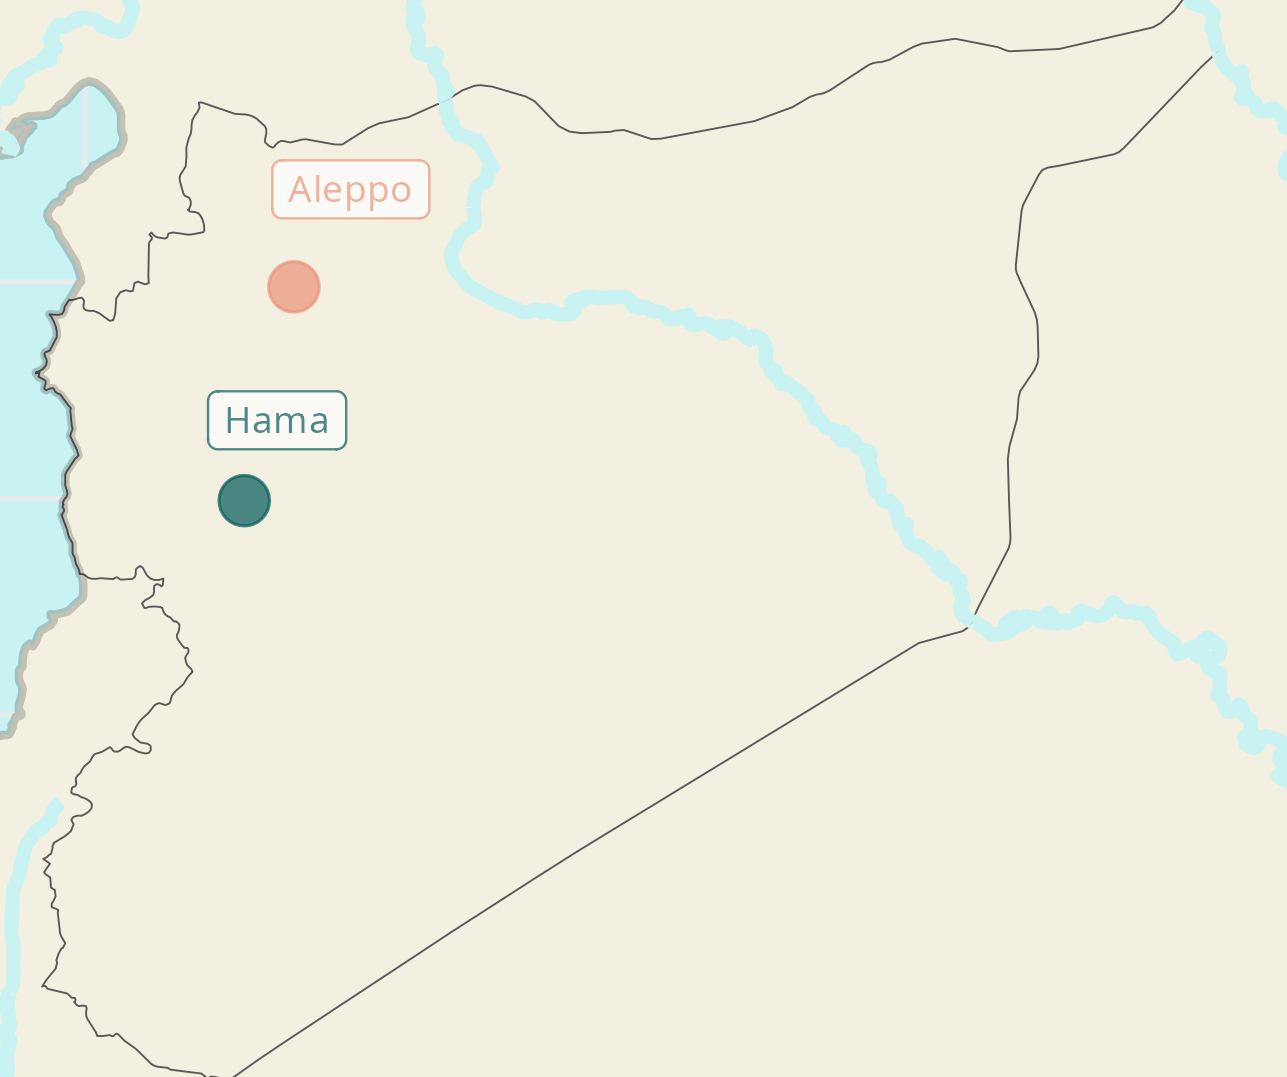
\includegraphics[width=0.8\textwidth]{../../../Mídia/Map02.png}
\end{flushright}

A inscrição HAMA 2 (\autoref{fig:hama2a}) está atualmente locada junto de HAMA
1 e 3 no Eski Şark Eserleri Müzesi, Istabul (no. 7890).

\begin{figure}[h]
	\centering
	\begin{subfigure}{0.49\textwidth}
		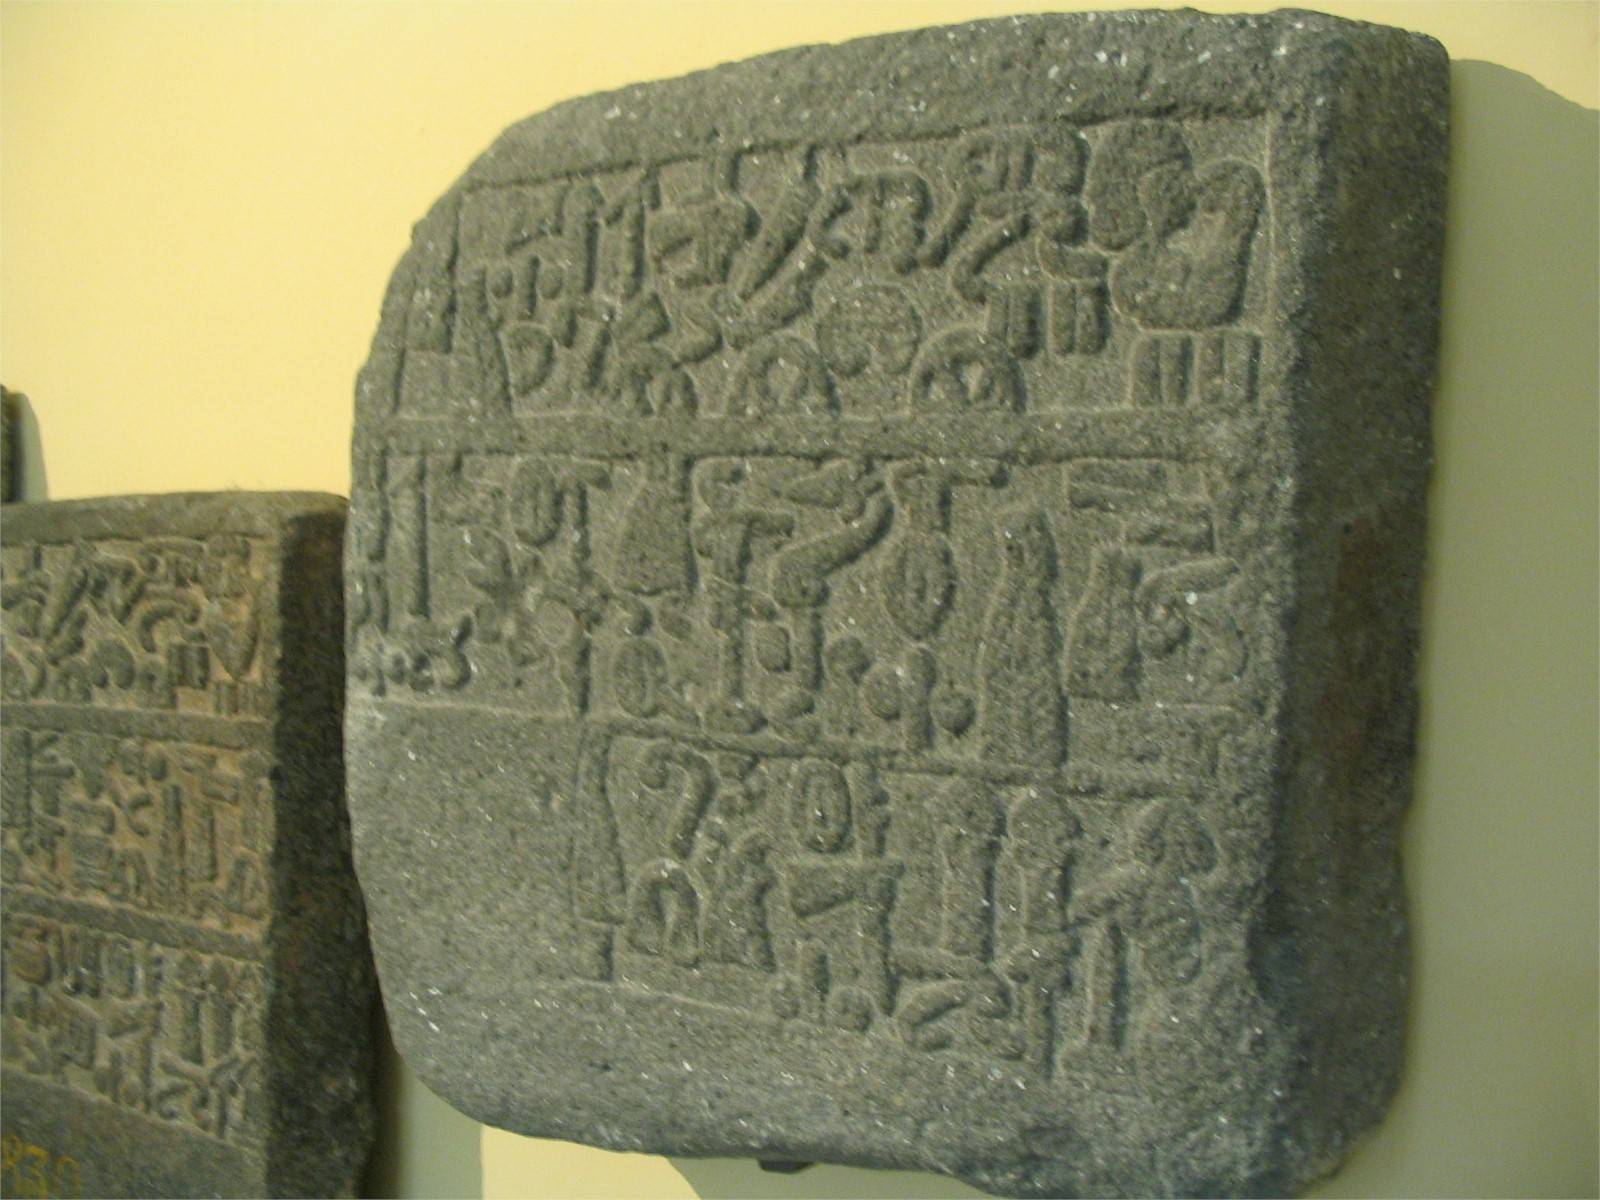
\includegraphics[width=\textwidth]{../../../Mídia/hama08.jpg}
	\end{subfigure}
	\begin{subfigure}{0.49\textwidth}
		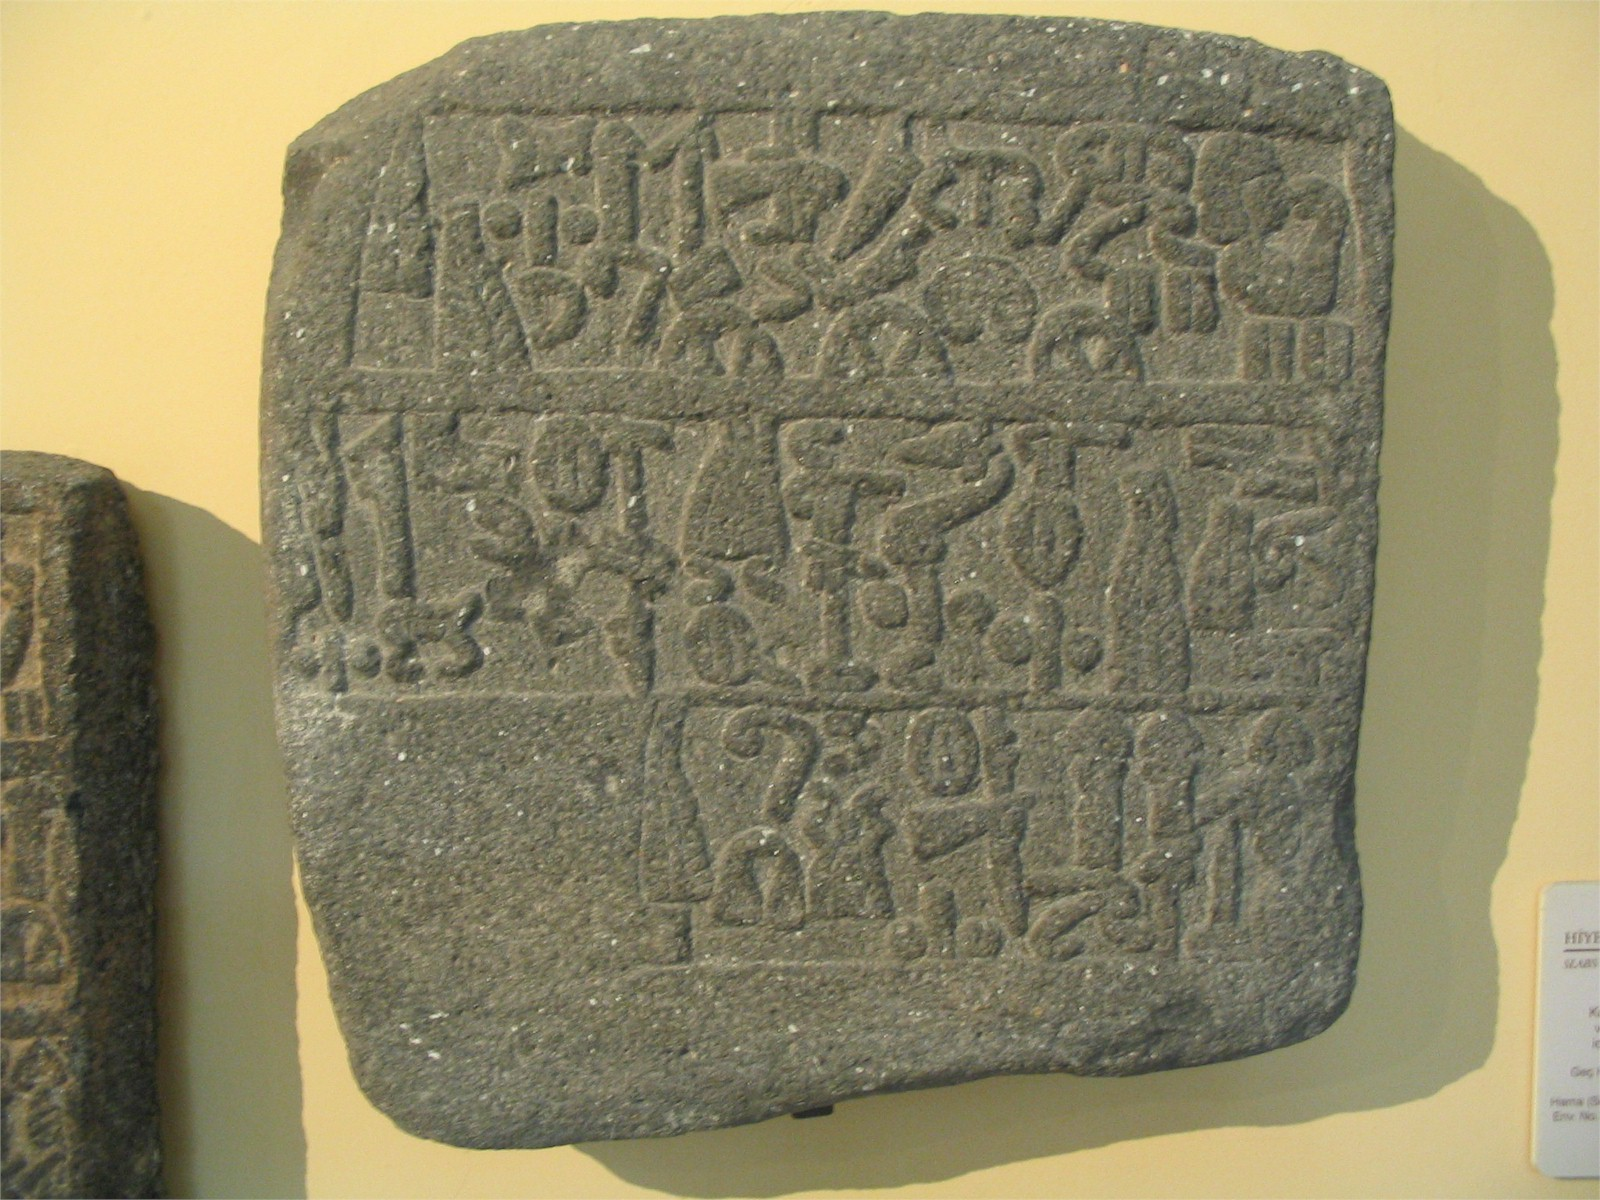
\includegraphics[width=\textwidth]{../../../Mídia/hama09.jpg}
	\end{subfigure}
	\caption[Inscrição HAMA 2]{Inscrição HAMA 2. Dimensões da inscrição:
		0.36\times0.31m.
		Imagens de Bora Bilgin, 2006,
		disponíveis em
		\href{https://www.hittitemonuments.com/hama/}{Hittite Monuments}.
		Edição e traçado em~\citeabbrev*{CHLI11}, pp.\ 411ff.\ e \emph{plates}
		221--2.
	}\label{fig:hama2a}
\end{figure}

\clearpage%


\begin{center}
	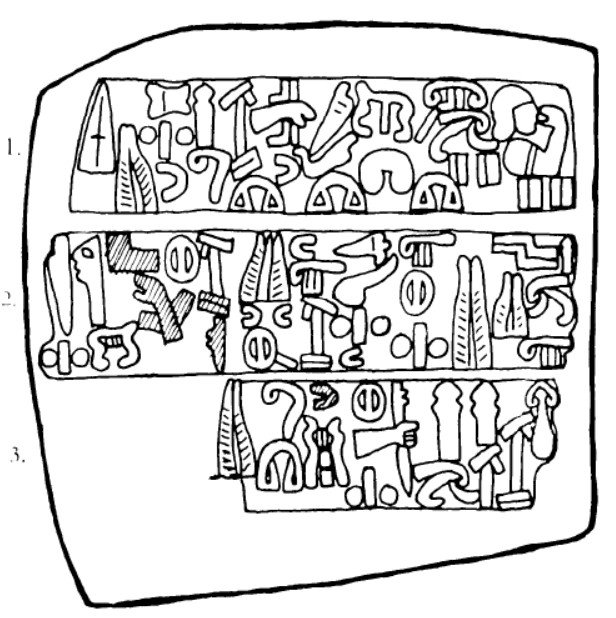
\includegraphics[width=0.85\textwidth]{../../../Mídia/hama14.jpg}
\end{center}

\ex.[]\ag.[1]\LARGE \luwiantrans{EGO-mi} \LARGE \luwiantrans{MAGNUS-ra-da-mi-sa}
\LARGE \luwiantrans{u-ra-hi-li-na-sa} \LARGE \luwiantrans{FILIUS-ni-za-sa}
\LARGE \luwiantrans{i-ma-tu-wa-ni REGIO} \LARGE \luwiantrans{REX}\\
EGO=mi MAGNUS-ra/i-da-mi-sa
u+ra-hi-li-na-sa FILIUS.\emph{NI}-za-sa
{i-ma-tu-wa-ni REGIO} REX\\
amu=mi Uradamis Urhilinas nimuwizas imatuwani hantawatis\vspace{10pt}
\bg.[2]\LARGE \luwiantrans{a=wa} \LARGE \luwiantrans{á-mu}
\LARGE \luwiantrans{AEDIFICARE-mi-ha} \LARGE \luwiantrans{za-a}
\LARGE \luwiantrans{<CASTRUM>-hara-ni-sà-za}
\LARGE \luwiantrans{la-ka-wa-ni-sà-ha-wa REGIO}
\LARGE \luwiantrans{FLUMEN.REGIO-da-i-sà}
\\
a=wa/i á-mu AEDIFICARE+\emph{MI}-ha za-' ``CASTRUM''-hara-ni-sà-za
{la-ka-wa/i-nis=ha=wa/i REGIO} FLUMEN.REGIO-da-i-sà\\
a=wa amu tamaha za harnisa=za | lakawanis=ha=wa hapadis\vspace{10pt}
\bg.[3]\LARGE \luwiantrans{REL-za}
\LARGE \luwiantrans{i-zi-da}
\LARGE \luwiantrans{a-tá-ha-wa}
\LARGE \luwiantrans{ni-ki-ma-sa REGIO}
\\
REL-za i-zi-i-da a-tá-ha-wa/i {ni-ki-ma-sa REGIO}\\
kwa=za izida || anda=ha=wa nikimas

\clearpage%

\ex.[]\ag.[1] amu =mi Uradamis Urhilinas nimuwizas imatuwani hantawatis.\\
\Pro{}1\Sg{} =\Refl{}. U.-\Com{}\Nom{}\Sg{} U.-\Com{}\Gen{}\Sg{} filho-\Com{}\Nom{}\Sg{}
imatuano-\Com{}\Nom{}\Sg{} rei-\Com{}\Nom{}\Sg{}\\
Eu sou Uradamis, filho de Urhilinas, rei imatuano.
\bg.[2] a =wa amu tamaha za harnisa=za,\\
\Conj{} =\Clt{} \Pro{}1\Sg{} construir-1\Sg{}\Pret{} \Pro{}\Neut{}\Acu{}\Sg{}
fortaleza-\Neut{}\Acu{}\Sg{}=\Clt{}\\
E eu (mesmo) construí esta fortaleza,
\bg.[||] lakawanis =ha =wa hapadis\\
L.\Com{}\Nom{}\Sg{} =\Conj{} =\Clt{} fluvial-\Com{}\Nom{}\Sg{}\\
\bg.[3] kwa=za izida,\\
\Rel{}\Neut{}\Acu{}\Sg{}=\Clt{} fazer-3\Sg{}\Pret{}\\
a qual o povo de Laka fez,
\bg.[] anda=ha=wa Nikimas.\\
dento=\Conj{}=\Clt{} N.\Com{}\Nom{}\Sg{}\\
E dentro [dela está] Nikima.

\subsection*{Notas}

\paragraph{Linha 1}
\textbf{amu=mi} `eu (sou)': o verbo \emph{as-} `ser, estar' é com frequência deixado
explícito em sentenças nominais e nestes casos costuma-se utilizar a
forma reflexiva do pronome.

\noindent\textbf{imatuwani} `imatuano, proveniente de Hama': em casos muito raros, a
desinência do nominativo singular comum não é expressa na grafia, algo que é
mais comum em inscrições majoritariamente logográficas. A série de inscrições de
Uradamis em Hama (1--3 e 6--7) não utilizam a desinência no gentílico
\emph{imatuwani-}.
Curiosamente, as inscrições de Urhilina, pai de Uradamis, HAMA 4,
RESTAN, QALʿAT EL MUDIQ e HINES,
também não empregam desinência de nominativo no gentílico e, em adição, não
inclui a desinência no nome próprio do rei.
HAMA 8, no entanto, também de Urhilina, emprega a desinência no gentílico, mas
não no nome do rei.
Outras inscrições escavadas em Hama, a saber, MEHARDE e SHEIZAR, empregam
regularmente as desinências.

\noindent\textbf{nimuwizas} `filho': por vezes, assume-se a existência de \emph{niza-}
`filho', um sinônimo de \emph{nimuwiza-} `filho', mas atualmente entende-se que
a grafia <FILIUS-ni-za-sa> e similares represente o logogram FILIUS com o
complemento fonológico \emph{NI} e /za-sa/ representem a fonologia da forma
subjacente, daí que transliteramos FILIUS.\emph{NI}-za-sa
(\citeabbrev*{CHLI3} \emph{ad loc.}).

\noindent\luwiantrans{REX} \textbf{= hantawatis} `rei': a forma sempre é escrita com \luwiantrans{REX} e
nunca é escrita com sua fonologia completa,
apenas com o final \emph{ti-}.\footnote{Raríssimas vezes, com \emph{-ta-}.}
Reconstrói-se a forma subjacente a partir do luvita cuneiforme
\emph{handawati-} `rei'.

\paragraph{Linha 2}
\textbf{amu} `eu': quando o pronome pessoal é utilizado, costuma-se entender que
seja para denotar algum tipo de ênfase, algo como `eu mesmo, fui eu que\ldots{}'.

\noindent\luwiantrans{AEDIFICARE-mi-ha} \textbf{= tamaha} `(eu) construí': note no
traçado da inscrição que \luwiantrans{mi} está \emph{em volta} da mão do
logograma \luwiantrans{AEDIFICARE}. Este uso é frequente para indicar que a
forma subjacente de um certo logograma contém em alguma parte de seu tema um
fonema /m/, independentemente do valor da vogal.\footnote{Por vezes, além
	do complemento fonológico anexado ao logograma, a sílaba /ma/ é representada
	por silabogramas: AEDIFICARE.\emph{MI}-ma-da = \emph{tamada} `ele construiu'
	(KARATEPE 2, §1).}

\noindent\luwiantrans{za-a} \textbf{= za' = za}: o sinal L.450 \luwiantrans{a} funciona
aqui de espaçador.
\textbf{harnisa=za}: \emph{=za} como partícula de dupla marcação do acusativo
neutro singular.

\paragraph{Linhas 2-3}
\textbf{la-ka-wa/i-nis=ha=wa/i REGIO} `povo de Laka': notar que o logograma
determinativo aparece no \emph{final} da escrita fonológica e após a cadeia de
clíticos.

\noindent\luwiantrans{FLUMEN.REGIO-da-i-sà} \textbf{= hapadis} `[terra] fluvial;
alagadiço': nas inscrições HAMA 1--3, parece que os escribas imatuanos,
para deixarem claro que uma sílaba /Ti/ contém uma oclusiva sonora /d/,
escrevem a sequência \luwiantrans{da-i} <da-i> ao invés de empregarem o
silabograma \luwiantrans{ti} <ti>, que poderia representar tanto /ti/ quanto
/di/. No resto do \emph{corpus}, a forma é regularmente escrita com
\luwiantrans{ti} <ti>.\footnote{
	Para uma interpretação contrária, ver~\citet{Simon2019}, que propõe que o
	sinal L.41 possa ter também o vocalismo em /i/, assim <da/i>.
}

\noindent\textbf{lakawanis\ldots{} hapadis} `povo da terra fluvial de Laka': sujeito da
oração relativa iniciada na linha seguinte por \emph{kwa{(n)}=za}.
O motivo da prolepse é incerto, mas pode-se argumentar que a troca de
sujeito\slash{}tópico de Uradamis para o povo de Laka a tenha motivado.

\noindent\textbf{kwa{(n)}=za} `a qual': o referente da relativa é \emph{harnisa=za}
[2].

\noindent\textbf{izida} `fez': o contraste feito entre \emph{amu tamaha} `eu (mesmo)
construí' e \emph{lakawanis hapadis kwa{(n)}=za izida} `o povo da região
fluvial de Laka que a fez' é bastante marcado tanto pela presença do pronome
pessoal quanto pela prolepse do sujeito da oração relativa.
O mesmo ocorre em todas as outras inscrições HAMA 1--3 e 6--7:
\begin{compactitem}
	\item HAMA 1: \emph{hurpadawanis hapadis kwa=za izida} `a qual o povo da região
	fluvial de Hurpada fez'
	\item HAMA 3: \emph{musanipawanis hapadis kwa=za izida} `a qual o povo da região
	fluvial de Musanipa fez'
	\item HAMA 6: \emph{kusunalanzi kwa=za iziyanta} `a qual os kussunalitas fizeram'
	\item HAMA 7: MONS \emph{labarnawanis hapadis kwa=za izida} `a qual o
	povo da região fluvial do monte Labarna fez'
\end{compactitem}

\noindent\textbf{anda=ha=wa} `e dentro [está]': as inscrições HAMA 1, 2 e 7
terminam com esta fórmula seguida de um topônimo.
A fortaleza não poderia cobrir a extensão necessária para conter todos os
territórios nomeados, de modo que se a interpretação for literal `dentro da
fortaleza está X', deve-se entender `dentro está parte da população de X',
talvez aquartelada para defender a fortaleza.
Outra interpretação possível é que em 1, 2 e 7, estejam sendo adicionados outros
povos à lista dos que fizeram, com o sentido `fortaleza a qual o povo Y fez,
\emph{incluindo} o povo de X'.


\begin{flushleft}
	\noindent \textbf{Transcrição}\\
	\noindent [1] \emph{amu=mi Uradamis Urhilinas nimuwizas imatuwani hantawatis.}\\
	\noindent [2] \emph{a=wa amu \mbox{tamaha} za harnisa=za,}\\
	\noindent [3] \emph{lakawanis=ha=wa hapadis kwa=za izida,}\\
	\noindent [4] \emph{anda=ha=wa \mbox{nikimas}.}


	\noindent \textbf{Tradução}\\
	\noindent [1] ``Eu sou Uradamis, filho de Urhilina, rei imatuano.\\
	\noindent [2] Eu mesmo construí esta fortaleza,\\
	\noindent [3] (e) a qual o povo de Laka fez\\
	\noindent [4] e dentro dela está Nikima.''
\end{flushleft}


\noindent\textbf{Vocabulário}
\begin{multicols}{2}
	\noindent \emph{amu-} (\emph{pron.1sg.}) eu\\
	\noindent \emph{anda} (adv.) dentro\\
	\noindent \emph{Uradami}- (NP com.) Uradamis\\
	\noindent \emph{Urhilina}- (NP com.) Urhilina\\
	\noindent \emph{hantawati}- (subst.com.) rei\\
	\noindent \emph{hapadi}- (adj.) fluvial\\
	\noindent \emph{harnisa}- (subst.neut.) fortaleza\\
	\noindent \emph{imatuwani}- (adj.) proveniente de Hama\\
	\noindent \emph{izi{(ya)}}- (v.t.) fazer, criar\\
	\noindent \emph{lakawani}- (adj.) proveniente de Laka\\
	\noindent \emph{nikima-}- (subst.com., topônimo) Nikima\\
	\noindent \emph{nimuwiza}- (subst.com.) filho\\
	\noindent \emph{tama}- (v.t.) construir
\end{multicols}



\backmatter%

\printbibliography%

\clearpage

\chapter*{Extras}

Incluo aqui todas as inscrições da fortaleza de Uradamis para aqueles que
quiserem tentar experimentar a leitura de textos por conta própria.
Os traçados e fotos das inscrições estão disponíveis no site
\href{https://www.hittitemonuments.com/hama/}{Hittite Monuments > HAMA}.
Comentários detalhados em~\citeabbrev*{CHLI11}, p.\ 411ff.



\vspace{20pt}
\noindent \textbf{HAMA 1}
\vspace{10pt}

\begin{parnumbersa}[]
	\raggedright%

	\large \luwiantrans{EGO-mi}\hspace{5pt}
	\luwiantrans{MAGNUS-ra-da-mi-sa}\hspace{5pt}
	\luwiantrans{u-ra-hi-li-na-sa}\hspace{5pt}
	\luwiantrans{FILIUS-ni-za-sa}\hspace{5pt}
	$[$\luwiantrans{i-ma-tú-wa-ni REGIO}\hspace{5pt}
					\luwiantrans{REX} $]$


	\large $[$\luwiantrans{a-wa}\hspace{5pt}
					\luwiantrans{á-mu}\hspace{5pt}
					\luwiantrans{AEDIFICARE-mi-ha}\hspace{5pt}
					\luwiantrans{za-a}$]$\hspace{5pt}
	\luwiantrans{<CASTRUM>-hara-ni-sà-za}\hspace{5pt}
	\luwiantrans{hu-ra-pa-da-wa-ni-sa REGIO}\hspace{5pt}
	\luwiantrans{FLUMEN-REGIO-da-i-sa}

	\large \luwiantrans{REL-za} \hspace{5pt}
	\luwiantrans{i-zi-i-da}\hspace{5pt}
	\luwiantrans{a-tá-ha-wa}\hspace{5pt}
	\luwiantrans{TONITRUS-HALPA-pa-wa-ni-zi REGIO}

\end{parnumbersa}

\vspace{10pt}
\hrule
\vspace{10pt}

\setcounter{parcount}{0}
\begin{parnumbersa}[]

	\raggedright%
	\itshape%

	\logo{EGO}-mi
	\logo{MAGNUS}+ra/i-da-mi-sa
	u-ra/i-hi-li-na-sa
	\logo{FILIUS}.NI-za-sa
	$[$i-ma-tú-wa/i-ni\logo{(REGIO)}
					\logo{REX}$]$

	$[$a-wa/i á-mu \logo{AEDIFICARE}+MI-ha za-'$]$ \logo{(``CASTRUM'')}hara/i-ni-sà-za
	hu+ra/i-pa-da-wa/i-ni-sa\logo{(REGIO)} \logo{FLUMEN.REGIO}-da-i-sa

	\logo{REL}-za i-zi-i-da a-tá-ha-wa/i \logo{TONITRUS.HALPA}-pa-wa/i-ni-zi\logo{(REGIO)}


\end{parnumbersa}

\vspace{10pt}
\hrule
\vspace{10pt}


\setcounter{parcount}{0}
\begin{parnumbersa}[]

	\raggedright%
	\itshape%
	amu=mi Uradamis Urhilinas nimuwizas $[$imatuwani hantawatis.$]$

	$[$a=wa amu tamaha za$]$ harnisa=za, Hurpadawanis hapadis

	kwa=za izida, anta=ha=wa Halpawaninzi.


\end{parnumbersa}

\vspace{10pt}
\hrule
\vspace{20pt}

\noindent \textbf{HAMA 3}
\vspace{10pt}

\setcounter{parcount}{0}
\begin{parnumbersa}[]
	\raggedright%
	\itshape%

	\large \luwiantrans{EGO-mi}\hspace{5pt}
	\luwiantrans{MAGNUS-ra-da-mi-sa}\hspace{5pt}
	\luwiantrans{u-ra-hi-li-na-sa}\hspace{5pt}
	\luwiantrans{FILIUS-ni-za-sa}\hspace{5pt}
	\luwiantrans{i-ma-tú-wa-ni}\hspace{5pt}
	\luwiantrans{REGIO}\hspace{5pt}
	\luwiantrans{REX}\hspace{5pt}
	\luwiantrans{a-wa}

	\luwiantrans{á-mu}\hspace{5pt}
	\luwiantrans{AEDIFICARE-mi-ha}\hspace{5pt}
	\luwiantrans{za-a}\hspace{5pt}
	\luwiantrans{<CASTRUM>-hara-ni-sà-za}\hspace{5pt}
	\luwiantrans{mu-sa-ni-pa-wa-ni-sà REGIO}\hspace{5pt}
	\luwiantrans{FLUMEN-REGIO-sà}\hspace{5pt}
	\luwiantrans{REL-za}\hspace{5pt}
	\luwiantrans{i-zi-i-da}


\end{parnumbersa}

\vspace{10pt}
\hrule
\vspace{10pt}


\setcounter{parcount}{0}
\begin{parnumbersa}[]
	\raggedright%
	\itshape%

	\logo{EGO}-mi
	\logo{MAGNUS}-ra-da-mi-sa
	u-ra-hi-li-na-sa
	\logo{FILIUS}.NI-za-sa
	i-ma-tú-wa/i-ni\logo{(REGIO)}
	\logo{REX}
	a-wa/i

	á-mu \logo{AEDIFICARE}+MI-ha za-' \logo{(``CASTRUM'')}hara/i-ni-sà-za
	mu-sa-ni-pa-wa-ni-sà\logo{(REGIO)}
	\logo{FLUMEN.REGIO}-sà
	\logo{REL}-za i-zi-i-da



\end{parnumbersa}

\vspace{10pt}
\hrule
\vspace{10pt}

\setcounter{parcount}{0}
\begin{parnumbersa}[]
	\raggedright%
	\itshape%
	amu=mi Uradamis Urhilinas nimuwizas imatuwani hantawatis.\ a=wa

	amu tamaha za harnisa=za, Musanipawanis hapadis kwa=za izida

\end{parnumbersa}

\vspace{10pt}
\hrule
\vspace{20pt}

\sloppybottom%
\clearpage

\noindent \textbf{HAMA 6}
\vspace{10pt}

\setcounter{parcount}{0}
\begin{parnumbersa}[]
	\raggedright%
	\itshape%

	\large \luwiantrans{EGO-mi}\hspace{5pt}
	\luwiantrans{MAGNUS-ra-da-mi-sa}\hspace{5pt}
	\luwiantrans{u-ra-hi-li-na-sa}\hspace{5pt}
	\luwiantrans{FILIUS-ni-za-sa}\hspace{5pt}
	\luwiantrans{i-ma-tú-wa-ni REGIO}\hspace{5pt}
	\luwiantrans{REX}\hspace{5pt}
	\luwiantrans{a-wa}\hspace{5pt}

	\large \luwiantrans{á-mu}\hspace{5pt}
	\luwiantrans{AEDIFICARE-mi-ha}\hspace{5pt}
	\luwiantrans{za-a}\hspace{5pt}
	\luwiantrans{<CASTRUM>-hara-ni-sà-za}\hspace{5pt}
	\luwiantrans{𔓻-ku-su-na-la-zi REGIO}\hspace{5pt}
	\luwiantrans{REL-za}\hspace{5pt}
	\luwiantrans{i-zi-ia-ta}


\end{parnumbersa}

\vspace{10pt}
\hrule
\vspace{10pt}


\setcounter{parcount}{0}
\begin{parnumbersa}[]
	\raggedright%
	\itshape%
	\logo{EGO}-mi
	\logo{MAGNUS}-ra-da-mi-sa
	u-ra-hi-li-na-sa
	\logo{FILIUS}.NI-za-sa
	i-ma-tú-wa/i-ni\logo{(REGIO)}
	\logo{REX}
	a-wa/i

	á-mu
	\logo{AEDIFICARE}+\emph{MI}-ha
	za-'
	\logo{(``CASTRUM'')}hara/i-ni-sà-za
	\logo{(``*218'')}ku-su-na-la-zi\logo{(REGIO)}
	\logo{REL}-za i-zi-ia-ta


\end{parnumbersa}

\vspace{10pt}
\hrule
\vspace{10pt}

\setcounter{parcount}{0}
\begin{parnumbersa}[]
	\raggedright%
	\itshape%
	amu=mi Uradamis Urhilinas nimuwizas imatuwani hantawatis.

	a=wa amu tamaha za harnisa=za, Kusunalanzi kwa=za iziyanta.


\end{parnumbersa}

\vspace{10pt}
\hrule
\vspace{20pt}


\noindent \textbf{HAMA 7}
\vspace{10pt}

\setcounter{parcount}{0}
\begin{parnumbersa}[]
	\raggedright%
	\itshape%

	\large \luwiantrans{EGO-mi}\hspace{5pt}
	\luwiantrans{MAGNUS-ra-da-mi-sa}\hspace{5pt}
	\luwiantrans{u-ra-hi-li-na-sa}\hspace{5pt}
	\luwiantrans{FILIUS-ni-za-sa}\hspace{5pt}
	\luwiantrans{i-ma-tú-wa-ni REGIO}\hspace{5pt}
	\luwiantrans{REX} \hspace{5pt}
	\luwiantrans{a-wa}\hspace{5pt}
	\luwiantrans{á-mu}\hspace{5pt}
	\luwiantrans{AEDIFICARE-mi-ha}\hspace{5pt}

	\large \luwiantrans{za-a}\hspace{5pt}
	\luwiantrans{<CASTRUM>-hara-ni-sà-za}\hspace{5pt}
	\luwiantrans{<MONS>-la-pa-ra-na-wa-ni-sa}\hspace{5pt}
	\luwiantrans{FLUMEN-REGIO-da-i-sà}\hspace{5pt}
	\luwiantrans{REL-za}\hspace{5pt}
	\luwiantrans{i-zi-i-da}\hspace{5pt}
	\luwiantrans{tú-ha-ia-ta-sa-ha REGIO}

	\large \luwiantrans{a-tá-ha-wa}\hspace{5pt}
	\luwiantrans{ha-ma-ia-ra-sa REGIO}

\end{parnumbersa}

\vspace{10pt}
\hrule
\vspace{10pt}


\setcounter{parcount}{0}
\begin{parnumbersa}[]
	\raggedright%
	\itshape%
	\logo{EGO}-mi
	\logo{MAGNUS}-ra-da-mi-sa
	u-ra-hi-li-na-sa
	\logo{FILIUS}.NI-za-sa
	i-ma-tú-wa/i-ni\logo{(REGIO)}
	\logo{REX}
	a-wa/i
	á-mu
	\logo{AEDIFICARE}+MI-ha

	za-'
	\logo{``CASTRUM''}hara/i-ni-sà-za
	\logo{``MONS''}.la-pa+ra/i-na-wa/i-ni-sa
	\logo{FLUMEN.REGIO}-da-i-sà
	\logo{REL}-za
	i-zi-i-da
	tú-ha-ia-ta-sa-ha\logo{(REGIO)}

	a-tá-ha-wa/i ha-ma-ia+ra/i-sa\logo{(REGIO)}



\end{parnumbersa}

\vspace{10pt}
\hrule
\vspace{10pt}


\setcounter{parcount}{0}
\begin{parnumbersa}[]
	\raggedright%
	\itshape%

	amu=mi Uradamis Urhilinas nimuwizas imatuwani hantawatis. a=wa amu tamaha

	za harnisa=za, Labarnawanis hapadis kwa=za izita,
	Tuhayatas=ha

	anta=ha=wa Hamayaras.


\end{parnumbersa}

\vspace{10pt}
\hrule
\vspace{20pt}



\begin{multicols}{2}[\noindent\textbf{Vocabulário}]
	\begin{hangparas}{1em}{1}
		\raggedright%
		\textbf{\emph{hamayarawani}-} (\emph{adj.}) \tabto{1em} proveniente de Hamayara\\
		\textbf{\emph{hurpadawani}-} (\emph{adj.}) \tabto{1em} proveniente de Hurpada\\
		\textbf{\emph{kusunala}-} (\emph{adj.}) \tabto{1em} proveniente de Kusuna\\
		\textbf{\emph{labarnawani}-} (\emph{adj.}) \tabto{1em} proveniente de Labarna\\
		\textbf{\emph{musanipawani}-} (\emph{adj.}) \tabto{1em} proveniente de Musanipa\\
		\textbf{\emph{tuhayata}-} (TO) \tabto{1em} Tuhayata\\
	\end{hangparas}
\end{multicols}

\vfill


\end{document}
